\chapter{緒論}
\label{chapter:intro}
\section{簡介}
% %IoT的重要性及地位
% 巨量資料所隱含的價值被挖掘後,物聯網受重視的程度也隨之提昇。其概念是串連人們身邊隨處可見的裝置及服務,整合原本分散的應用使其發揮更高的價值。
% %IoT的困難
% 嶄新的商業模式及應用需要分佈大量的感測器以提高覆蓋率,這使得整個物聯網系統的安全性、可靠度、負載率、產出及連接性都受到巨大的挑戰。對於一個延遲靈敏度高的服務而言,建構一
% 個高可靠度及效能表現穩定的系統將直接影響其服務的品質。

%Fog computing的特性及好處
霧運算繼承並且擴展雲端運算的特性及優勢,包含低延遲、分散式架構、機動性,上述特性使其能支援大量的感測器、無線傳輸存取及即時串流服務 \cite{bonomi_2012}。其優異的特性適合建構
高效的物聯網相關應用。
%Fog computing的必要性
例如智慧電網就需要建置大量的智慧電錶作為感測器,並且即時監測、回傳用電資訊至伺服器以進行下一步的運算 \cite{yi_2015}。若智慧電網系統是以霧運算架構為其基本建置結構,整體智慧
電網就可視為許多小型智慧電網群集的集合。用電資料將區域性的運算並即時回傳,需要整合性的做大量運算時才會回傳至運算中心以大型伺服器運算。此舉降低集中式伺服器的負載,同時享有
靈活調度運算資源的好處。

%Fog computing的分配是個問題
享有霧運算系統帶來的好處之前,要先解決其階層型的分散式架構的配置問題。配置伺服器將直接影響整體霧運算系統完成後的效能以及成本。霧運算伺服器將依據其配置位置調整服務,例如針
對區域性的需求客製化該區伺服器提供的應用,並在各霧運算群集中配置足夠的運算資源以就近服務終端使用者 \cite{luan_2015}。
%此分配問題是NP-hard問題
霧運算遇到的配置問題為如何找到一個資源配置的方案,使得各資源間的連線達成低延遲、低成本、高覆蓋率且能滿足各階層的運算需求量。此類型問題可被轉變為度受限最小生成樹
(degree-constrained minimum-spanning tree; DCMST)問題 \cite{kim_2015}。而在兩個以上的度限制下尋找DCMST是已知的NP-hard問題 \cite{narula_1980},故霧運算分配問題也是NP-hard
問題。

%NP-hard就用啟發式解決
目前NP-hard問題還沒有有效的方法可以在合理的時間內找到最佳解。所以此類問題通常會轉而在合理時間內,最大程度的找尋近似最佳解。相較於最佳化演算法或疊代法,超啟發式
(metaheristic)演算法雖然無法保證提供全域最佳解,但保證能在運算時間有限的情況下,對最佳化問題提供足夠好的區域最佳解。
\\
\\

\section{研究動機}
%應用到霧運算分配問題會有些問題
霧運算系統分配問題應用於智慧電網、工業4.0等環境中,因應大量的終端使用者,需要建置非常大量的感測器、邊緣運算伺服器以及霧運算伺服器。而運算產生的巨量資料也需要在各霧運算群
集中分配閘道器。此環境下的資源配置就形成一個巨大解空間的最佳化問題。
%啟發式演算法能解決小型的分配問題,針對大解空間的問題做不好
超啟發式演算法之所以無法保證提供全域最佳解的原因在於其尋優策略的特性。其核心想法是隨機產生一或多組初始解,藉由疊代從初始解開始探索解空間。而每次疊代都會保留原本解的部份特
徵,期望此特徵是構成最佳解的子特徵。但若保留下的特徵是區域最佳解的特徵將使得最終結果落到區域最佳解的可能性上升。在解空間較小的分配問題上,區域最佳解的數量較少,尋優過程中
也較容易均勻的探索整個解空間。傳統的超啟發式演算法如基因演算法(genetic algorithm; GA) \cite{holland_1962}、模擬退火(simulated annealing; SA) \cite{kirkpatrick_1983}、粒
子群最佳化演算法(particle swarm optimization; PSO) \cite{kennedy_1995}等都能提供良好的尋優效果。針對解空間大的最佳化問題,傳統超啟發式演算法會因為區域最佳解數量龐大抑或
沒有均勻的在解空間內尋優,而無法在合理的時間內提供夠好的區域最佳解。

% 即便某些演算法有一定的機率透過暫時接受較差解的方式試圖跳出該區域最佳解,但仍舊無法解決均勻的搜尋整個解空間的問題。若以跳出區域最佳解的方式面對龐大數量的區域最佳解,也只
% 會使得疊代次數增加。

%大解空間的問題有幾種策略
超啟發式演算法面臨此問題的策略主要都是增加搜尋多樣性。例如增加候選解數量以提高每次疊代可以搜尋區域最佳解的數量,並藉由交換各區域最佳解的特徵,嘗試組合出更加優秀的解。雖然
這種作法的確提昇解的品質,但在交換各區域最佳解的特徵的同時,搜尋多樣性的特性也隨之消失。各候選解容易漸漸朝向同樣區域尋優,疊代後期容易花費大量計算資源在重複的區域而無法進
一步得到新的最佳解。
%SE可以對大解空間做得不錯
Tsai \cite{tsai_2015}提出的搜尋經濟學演算法(search economics)針對上述問題發展一套基於切割解空間的框架,在切割的子解空間內依據其潛力投放搜尋資源。其主要目標是增加搜尋多
樣性且避免後期搜尋資源的浪費。不論在疊代前期抑或後期,搜尋資源將藉由該框架的分配而均勻的在分割後的解空間中搜尋。
\\
\\
\\
% 本論文將以擅長在大型解空間尋優的搜尋經濟學演算法解決此一配置問題。
\section{貢獻}
本論文提出一個基於搜尋經濟學演算法的霧運算系統配置演算法。在運算資源需求驟增的物聯網環境中,利用搜尋經濟演算法不易落入區域最佳解的特性解決配置問題。本論文主要貢獻分為以下
三點:
\begin{enumerate}[\hspace{2em}(\xCJKnumber{\arabic{enumi}})]
    \item 將搜尋經濟學演算法切割解空間的機制融合霧運算系統階層型的分散式架構的特性,對解空間進行有意義的切割。
    \item 基於搜尋經濟學演算法定義的兩種不同搜尋資源制定兼容貪婪性及搜尋多樣性的搜尋策略。
    \item 新增的貿易運算子改良搜尋資源在解空間中探索的機制,針對尚未收斂的區域加強搜尋以增進搜尋效率。
\end{enumerate}
以上三點改良使搜尋經濟學演算法在霧運算系統配置問題中能夠加強其搜尋廣度、深度、持續性及搜尋效率。相較於基於規則的最佳優先演算法、早期提出的基因演算法以及近期改良的離散猴群
基因演算法、離散猴群演算法,本論文在衡量成本、覆蓋率、傳輸延遲以及服務需求的綜合評量指標獲得更佳的結果。

\section{論文架構}
如圖 \ref{fig:thesis-arch},第二章首先整理相關問題定義,將實際的霧運算系統配置問題釐清。量化在霧運算系統內影響配置結果的重要指標,並定義實際計算方法。接著說明一個基於規則的演算法、一個早期的最佳化演
算法以及兩個近年針對類似分配問題的改良型演算法。詳細探討上述演算法原理以及在複雜解空間下的缺點。第三章將針對搜尋經濟學演算法深入探討,將分別介紹演算法中重要的運算子運作原
理及特性。對於改良的機制進行步驟及原理說明。第四章介紹實驗環境、測試資料集產生方法及資料集特性。演算法參數調整過程、實驗結果呈現及說明。第五章總結本篇論文結果,探討不足之
處作為未來改良方向。
\begin{figure}[H]
    \centering
    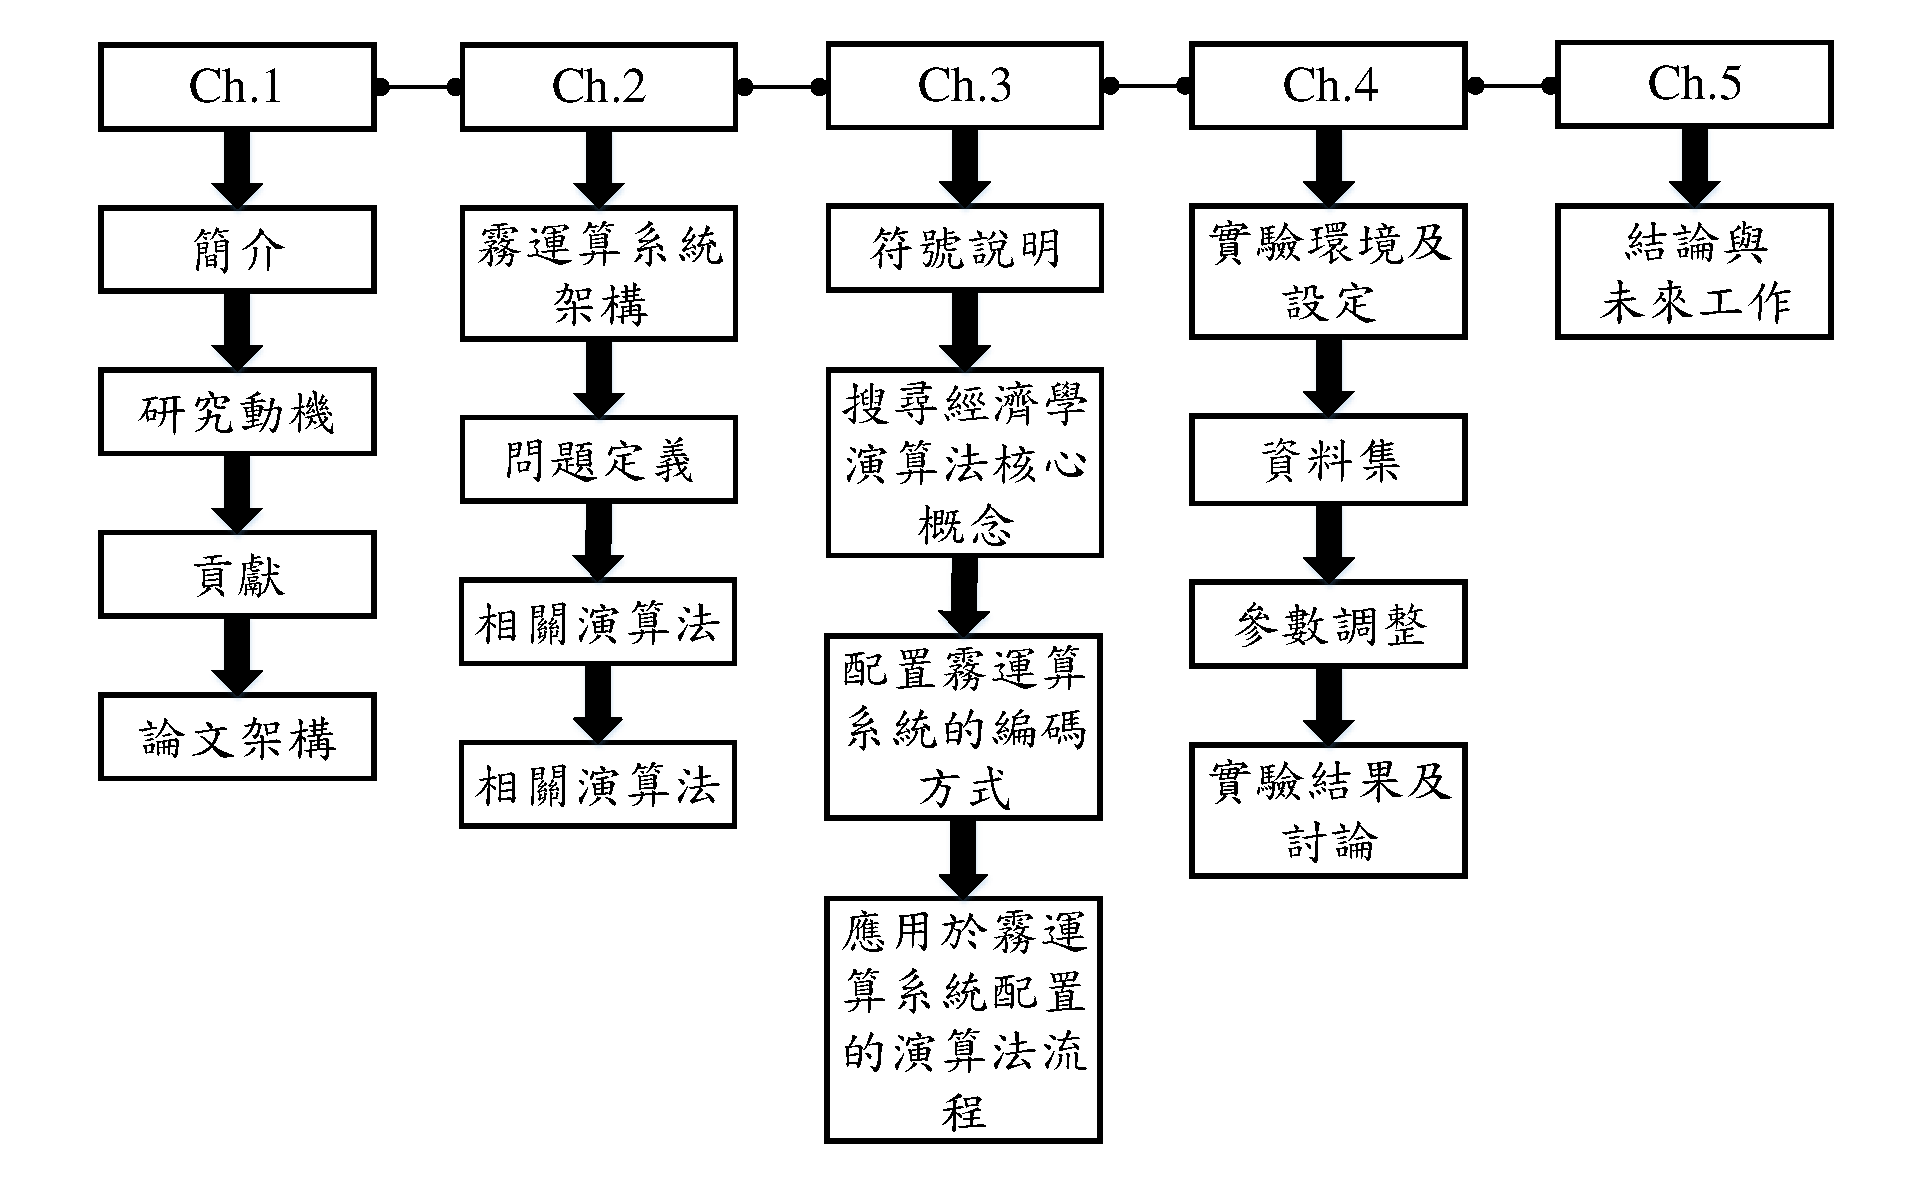
\includegraphics[height=!,width=1\linewidth,keepaspectratio=ture]
    {figures/thesis_arch}
    \caption[論文架構圖]{\normalsize 論文架構圖}
    \label{fig:thesis-arch}
\end{figure}

